% ##################################################################################################################
\chapter{Seoul}
\label{ch:seoul}
\hfill \textbf{Authors:} Seungjae Lee, Atizaz Ali

\editdone{This text has undergone the professional edit. Please no grammatical changes anymore! They are most-probably wrong.}

% ##################################################################################################################
The \gls{matsim} model of \gls{sma} was developed in 2012, as a result of long-term research collaboration between the University of Seoul (Prof.\ Seungjae Lee) \& \gls{eth} Zürich (Prof.\ Kay W.\ Axhausen). The model was updated yearly and demand was generated based on 2012 \gls{hhtsd}. Demand statistics (input) are summarized as follows. 

Study area was the \gls{sma} (Gyeonggi-do province, with emphasis on the Seoul Metro,  comprised of 25\,main administrative districts). A population synthesizer was developed to generate the \gls{matsim} input demand, based on \gls{hhtsd} 2012. Total population of \gls{sma} was 21.5\,million; therefore, a 10\,\% sample was generated and simulated (2.15\,million agents). A detailed nodes and links network was generated, capturing all details (16\,384 nodes and 32\,768 links) for railways, highways, arterials, pedestrians, expressways and bus-only lanes. \gls{emme2} network was converted to \gls{matsim} format. The 2012~Korean Transport Database was utilized to generate transit schedules and vehicle definitions, according to bus types, railway and metro lines. Total number of routes was 1\,317 (contained regional buses, inter-city buses, feeder line buses and metro lines, etc.). In collaboration with \gls{senozon}, a more realistic door-door demand was generated in Seoul City in July, 2014. Data source was the Korean \gls{gis} department.

In Seoul, \gls{matsim} has been widely used for various research purposes to aid policy evaluation \citet[e.g.,][]{KimEtAl_IJHE_2012, LeeAli_unpub_IWUTSCD_2014}.

A master's thesis on transit demand generation and calibration using smart card data in \gls{sma} is currently underway by this chapter's second author, sequenced as follows. A video is available from the authors on request.
%
\begin{itemize}\styleItemize
\item Data mining (trimming off non-useful data)
\item	Converting disaggregate transactions (\gls{od}) to individual trips and trip segments based on user \lstinline|ID|
\item	Activities inference and assignment in \gls{spss} database
\item	Generating transit demand (\gls{matsim} input format)
\item	Updated transit network \& schedule for running the simulation
\item	Model calibration (in process)
\end{itemize}
%
\gls{matsim} tutorials were also presented during the fall semester~2014 to help Department of Transportation Engineering undergrad and grad students gain a thorough working knowledge of \gls{matsim}.

\createfigure%
{Seoul scenario}%
{Seoul scenario}%
{\label{fig:seoul}}%
{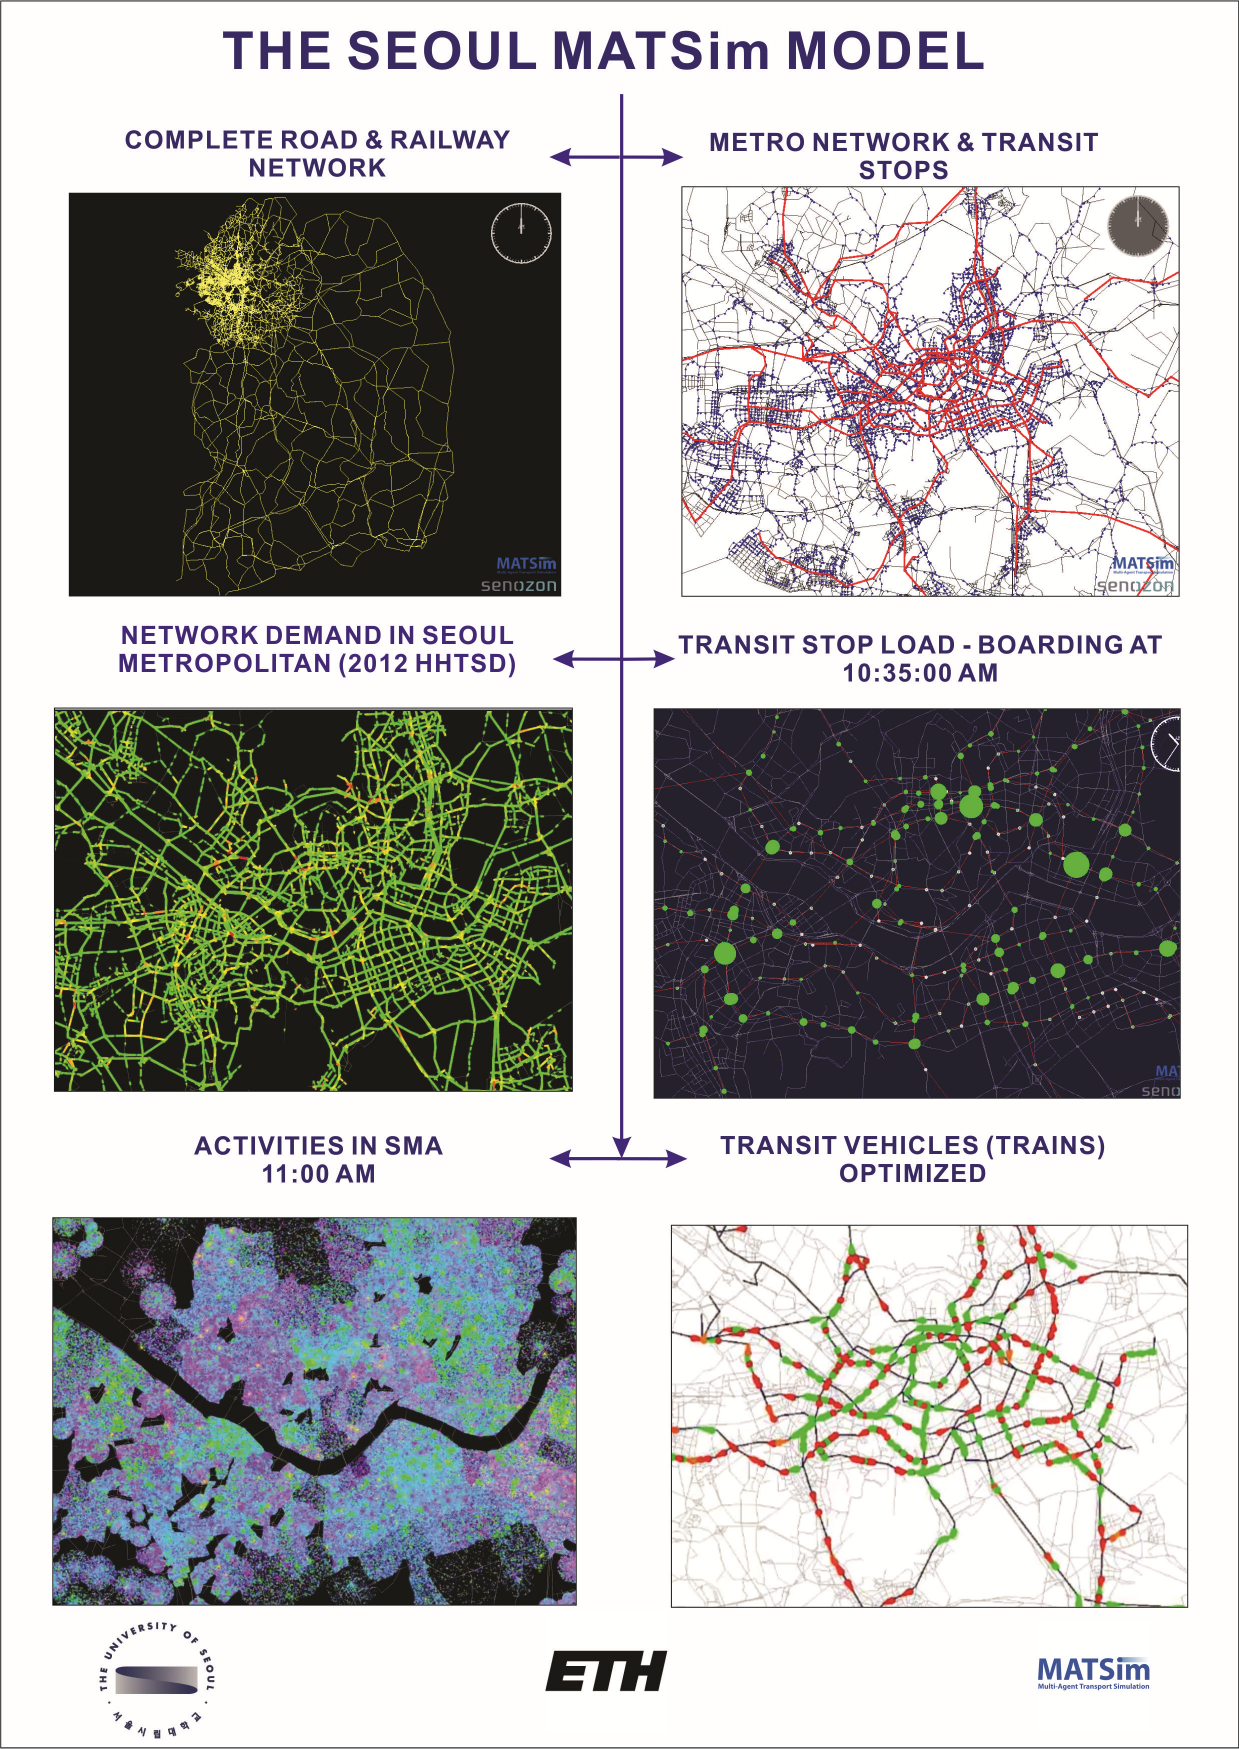
\includegraphics[width=0.99\textwidth, angle=0]{scenarios/figures/seoul}}%
{}

% ##################################################################################################################
 
 
